\documentclass[11pt,letterpaper ,oneside ]{book}
\usepackage{graphicx, color}
\usepackage{geometry}
\usepackage{url}
\usepackage{subfig}
\usepackage{amsthm}
\newtheorem{definition}{Definition}
\newcommand{\red}[1]{{\color{red}{#1}}}
\usepackage[]{algorithm2e}

\begin{document}

	\begin{titlepage}
	
	\newcommand{\HRule}{\rule{\linewidth}{0.5mm}} % Defines a new command for the horizontal lines, change thickness here
	\center % Center everything on the page
	
	%----------------------------------------------------------------------------------------
	%	HEADING SECTIONS
	%----------------------------------------------------------------------------------------
	
	%\includegraphics[width=\linewidth]{uvaENG}\\[2.5cm]
	\textsc{\Large MSc Artificial Intelligence}\\[0.2cm]
	\textsc{\Large Master Thesis}\\[0.5cm] 
	
	%----------------------------------------------------------------------------------------
	%	TITLE SECTION
	%----------------------------------------------------------------------------------------
	
	\HRule \\[0.4cm]
	{ \huge \bfseries \red{Designing custom inconsistent knowledge graphs}}\\[0.4cm] % Title of your document
	\HRule \\[0.5cm]
	
	%----------------------------------------------------------------------------------------
	%	AUTHOR SECTION
	%----------------------------------------------------------------------------------------
	
	by\\[0.2cm]
	\textsc{\Large \red{Thomas de Groot}}\\[0.2cm] %your name
	\red{11320303}\\[1cm]
	
	
	%----------------------------------------------------------------------------------------
	%	DATE SECTION
	%----------------------------------------------------------------------------------------
	
	{\Large \today}\\[1cm] % Date, change the \today to a set date if you want to be precise
	
	\red{36 EC}\\ %
	\red{September 2018 - March 2019}\\[1cm]%
	
	%----------------------------------------------------------------------------------------
	%	COMMITTEE SECTION
	%----------------------------------------------------------------------------------------
	\begin{minipage}[t]{0.4\textwidth}
		\begin{flushleft} \large
			\emph{Supervisor:} \\
			\red{Dr \textsc{Stefan Schlobach } }% Supervisor's Name
		\end{flushleft}
	\end{minipage}
	~
	\begin{minipage}[t]{0.4\textwidth}
		\begin{flushright} \large
			\emph{Assessor:} \\
			\red{Dr  \textsc{Joe Raad}}\\
		\end{flushright}
	\end{minipage}\\[2cm]
	
	%----------------------------------------------------------------------------------------
	%	LOGO SECTION
	%----------------------------------------------------------------------------------------
	
	\framebox{\rule{0pt}{2.5cm}\rule{2.5cm}{0pt}}\\[0.5cm]
	%\includegraphics[width=2.5cm]{figure}\\ % Include a department/university logo - this will require the graphicx package
	\textsc{\large \red{institute name}}\\[1.0cm] % 
	
	%----------------------------------------------------------------------------------------
	
	\vfill % Fill the rest of the page with whitespace
	
\end{titlepage}
\pagenumbering{roman}
% Writing of the report


\newpage
\chapter*{Abstract}

\newpage
\tableofcontents
\newpage
\pagenumbering{arabic}

% Rewriting titles to better fit the method

\chapter{Introduction}\label{Introduction}
\section{Motivation}
\textit{Background}. Blaise Pascal once said, "A contradiction is not a sign of falsity, nor the lack of a contradiction a sign of truth." Large amounts of data has been made available for everyone to use and Multi-billion facts, also called statements or triples, for a linked-data dataset being the standard in stead of the exception. We are sitting on a large amount of open data, but the problem however is that we do not know if all the facts available to use can be considered as the truth. We know that data is inherently dirty and it is known that finding new facts from the data is impossible if the data holds facts that are contradicting each other. While there is active development in solving the problem of contradictions in datasets by ignoring the contradictory facts and still use the rest of the "true" facts to still find new information that is hidden in the dataset. This method however, would still miss facts that could have been found if we could have removed the contradictory facts and used a datasets that is devoid of contradictions. So while a contradiction is no sign of a false dataset, a lack of contradictions would certainly be a step in the right direction to the truth. The only challenge is then to find if it is the correct truth!\\

\textit{Motivation}. Finding and removing contradictions from datasets in a simple and systematic way will have a number of benefits. Firstly we could study the types of mistakes that have been made in the datasets, and how these mistakes are made, by automatic algorithms, or by people in the process. This could help us clean problems by the source, the generation of the data, in stead of later in the process, during the cleaning. 
Secondly we can generalize the contradictions we have found and design blueprints that can be used to describe groups of contradictions, that can be applied to different datasets. Thirdly, we could use the found contradictions to analyze existing datasets. We can for example use the blueprints to find if there are contradictions in other datasets as well, and we could even count the amount to contradictions to analyze the datasets further. 
Finally, we can use the contradictions now that we understand them, to build benchmarks designed to test tools, that require large datasets with known characteristics.\\

\textit{Method} In this work, we developed a method of extracting contradictions from linked datasets. We call these generalised contradictions `anti-patterns', as these contradictions can be seen as common mistakes made in dataset. Most commonly used in software design, http://wiki.c2.com/?AntiPattern, describes an anti-pattern as a bad solution for a problem. We describe a formal notion of `anti-patterns' in chapter \ref{AntiPatternDefinition}.\\

For the extractions of the `anti-patterns' we have designed an extraction pipeline that can extract `anti-patterns' for an arbitrary, inconsistent linked-data dataset can retrieve the `almost' complete set `anti-patterns'. We show this by retrieving such `anti-patterns' from the LOD-a-lot\cite{JavierD:2017} a dataset containing 28 billion facts. We also use the set of `anti-patterns' we have found in the LOD-a-lot as input for the two implementations we designed. The two implementations we designed are, analysis for inconsistent knowledge graphs and a sampling method, and these implementations make extensive use of the found `anti-patterns'. 

\section{Research questions}
\textit{Research questions}. The main research goal of this work is the task if we can discover a effective method of finding contradictions and generalize the contradictions we found into `anti-patterns'. In the above section we already described our method informally. To formalise our we wrote down three research questions that form this paper.

\begin{itemize}
	\item \textbf{RQ1}: Can we describe and define a formal definition for general contradiction patterns, where general contradiction patterns are inconsistent subgraphs which are persistent throughout all natural knowledge graphs?
	\item \textbf{RQ2}: How can we retrieve the general contradiction patterns that have occurred in natural knowledge graphs? 
	\item \textbf{RQ3}: What classifications are there which can classify groups of general contradiction patterns? And what main characteristics can describe the classes of contradiction patterns best? Can we use these commonalities to give better qualitative and quantitative information about the graph?
	\item \textbf{RQ4}: Are there methods, or can we design methods that could benefit from using general contradiction patterns in their algorithm? 
	\begin{itemize}
		\item Are we able to improve analytics about contradictions for large linked datasets, by giving qualitative and quantitative information about a linked datasets?
		\item Can we use the anti-patterns, to build benchmarks. Benchmarks that have been sampled from large, but inconsistent datasets with general contradiction patterns. Would it be possible to keep the sampled characteristics invariant from sampling?
	\end{itemize}
\end{itemize}

\section{Contribution}
\textit{Experiments and implementations}. We test our extraction pipeline on two points, firstly if it is possible to retrieve all `anti-patterns' from a linked dataset. This is done by using a benchmark dataset, the "pizza-ontology". The "pizza-ontology" is a dummy dataset that holds only a small number of facts and a few contradictions, simple enough to check by hand. Secondly we test our extraction pipeline on the LOD-a-lot. One of the largest open datsets, we use the `anti-patterns' from this dataset as input for the later parts of our experiment.\\

Finally we have selected two implementations to evaluate our method with real-world examples. Firstly, we have designed a system that can analyse linked datasets. The system retrieves `almost' all the  `anti-patterns' based on contradictions in the LOD-a-lot, and calculates the number of times the `anti-patterns' occur in the linked datasets. Then, the system return a detailed report of characteristics of linked datasets.
Secondly, we show the implementation that samples a linked dataset and then generates sample of the original datasets that can be tweaked with a user-specified sample-size and the number of contradictions per `anti-patterns'. \\

\textit{Findings}. We have tested our pipeline by extracting an `almost' complete set of `anti-patterns' from the LOD-a-lot\cite{JavierD:2017}, which we made available >>LINK<<. We developed a set of characteristics that can be used to describe `anti-patterns' more consisely. 
We show that there is a correlation between the size of the `anti-pattern' and the amount of different `anti-patterns'. 
We tested two implementations by processing a set large knowledge graphs, DBpedia\cite{DBpedia}, and YAGO\cite{YAGO}.
We found that the `anti-patterns' give us a more detailed explanation to about the contradictions in an inconsistent knowledge graph. 
We show how the characteristics change between the datasets with different contradictions occur in different knowledge graphs. We also show that the  distribution of `anti-patterns' remains equal in all samples knowledge graphs. 
Secondly, we show that the sampled knowledge graphs match the set characteristics given by the user, and also match the characteristics of the original knowledge graph.\\

\textit{Contributions}. 
The main contributions in this works, with respect to the research questions can be described in threefold.
\begin{itemize}
	\item Firstly, we give a formal definition of `anti-patterns' we use to describe common occurring generalised contradictions that we found in the linked datasets. We use these definitions throughout this work to describe the generalized patterns.
	\item Secondly, we design an extraction pipeline that can extract `anti-patterns' from any arbitrary knowledge graph, we show that this method works by extracting "almost" all contradictions. We made all the `anti-patterns' available to use on the web.
	\item Thirdly we show that `anti-patterns' can be used to analyse inconsistent knowledge graphs and to systematically sample inconsistent knowledge graph.
\end{itemize}

\section{Outline}
 The second and third chapter explain the work that this paper is based on, as well as give some background to the reader about the definitions that we use in this work. In the method, we explain more in detail how the method of `anti-pattern' retrieval works. Section 6  showcases the possible applications that make extensive use from the `anti-pattern' that we retrieved in the method. In section 7 we show the experiments that test our hypotheses, we set in the introduction, and analyse the results. We conclude with a conclusion, with an extension of future work.

\newpage
\chapter{Background}\label{Background}
In this chapter, we introduce the set of essential preliminary concepts that are needed to understand the research that we present in this work. To help the reader, we also introduce a set of examples that are used in this paper to help the reader understand.

\section{Knowledge graph elements}\label{graphElements}
Knowledge graphs are the basis of some of the most advanced systems, Google for example uses a knowledge graph to enchance its search results, with other information about the search question shown in the box next to the question. Searching for "Frank van Harmelen", not only shows the results, but also shows other information about him, without even having to click on the wikipedia link. The information that is shown, comes from the knowledge graph Google has build. But what is exactly a knowledge graph?

\textit{RDF triple}. To understand how a knowledge graph works we first need to introduce the RDF triple. RDF triples are the building blocks of knowledge graphs and are used to describe facts. These facts can be anything. For example, Lisa owns Sam, or Sam is of type Rabbit, Sam is Brown.  The challenge is that each RDF triple consists out three elements.
These three elements are $<$Subject$>$, $<$Predicate$>$, and $<$Object$>$. Where the subject and the object are two entities and the predicate is the link between them, describing the relation between the two entities. 

There are however a few problems with writing $<$Lisa$>$ $<$owns$>$ $<$Sam$>$ . What if there is more than one Sam? To counter this we use (Uniform Resource Identifier) or otherwise known as URI to define an entity. A URI is a set of characters that unambiguously identifies an abstract or physical resource. Lisa would become $<$https://data.persons.com/world/Europe/Netherlands/amsterdam/122341$>$ $<$https://names.org/hasname$>$ "Lisa". Where this statement links the identifier, to the name Lisa. Now every time Lisa is mentioned the long identifier is used. 
The second problem that needs solving is the standardization of the relation description, such that each relation type has an unique meaning, which can be related back to a language describing this meaning. This also opens the gate for reasoning because if we know the meaning of the fact we can learn new facts. Before we can get to that languages need to be defined. Starting with RDF, RDFs, and OWL.

\textit{RDF} \cite{rdfPrimer:2014} stands for \textbf{r}esource \textbf{d}escription \textbf{f}ramework and is a method of storing data in triple format. These statements, consisting out of the $<$Subject$>$, $<$Predicate$>$, $<$Object$>$. can hold different types. The subject can be defined as a URI or a blank node. The predicate represents the relation between the Subject and the Object, and is always defined as a URI. finally the object is the second resource, this can be a URI, blank node or a literal.
RDF is designed to exchange information between processes and applications without the intervention of humans. The goal was to build a framework that is designed link resources without having to add in expensive parsers to convert the information to the correct format every time a new process is added which wants to use the information.\\

\textit{RDFS} \cite{RDFSchema:2014} Extending to this is RDFS, this the RDF schema, with this schema we can allow to define ontologies within RDF. It can be used to give structure to the RDF ontology. Both RDF(s) and OWL are ontologies from the semantic web community. But they are special in the sense that these languages can be used to reason with. thus making it possible to infer new facts from the knowledge of other triples.\\

\textit{OWL}\cite{OWLPrimer:2012}, the Web Ontology Language, designed to represent the language that can describe things and set of things well with regards to relations. But not only that, in OWL it is also possible to reason with that knowledge and make implicit knowledge explicit, for example reason that a subClassOf(Car, Audi) and subClassOf(Audi, A1 Sportsback). This makes it possible to reason that subClassOf(Car, A1 Sportsback) is also a type of relation that exists. 

\textit{Knowledge graph}. 
Now that the building blocks of a knowledge graph are covered it is time to introduce the knowledge graph. A knowledge graph can be seen as a part of a knowledge based system. Where the knowledge base stores all the statements, which represent the facts about the known world. The second part of the knowledge based systems are is the reasoner, which will be discussed in a later part of the this chapter. A knowledge graph consist out of a large amount of RDF triples, also known as statements or facts.

\textit{Basic Triple Pattern}. The problem with RDF triples is that each triple is instantiated, meaning that all triples have a value, which can be a URI, or a literal,  a fixed value in the statements, such as "Lisa", "12", "True". 
To have the ability to generalise within a knowledge graph we use Basic triple patterns(BTP). BTPs can be seen as RDFtriples, but where it is possible to change one, two or all three elements from the RDFtriple into variables. With an uninstantiated BTP, we can ask a question to the knowledge graph and retrieve instantiated BTPs back. Alternatively, we can check with an instantiated BTP if it exists in the knowledge graph.\\

\textit{Basic Graph Pattern}. A basic graph pattern (BGP) is a set of basic triple patterns and forms the basis of query matching. The basic graph pattern
can consist out of BTPs that are connected, either through $<$Subject$>$ and $<$Subject$>$, $<$Subject$>$ and $<$Object$>$, or $<$Object$>$ and $<$Object$>$.
Alternatively, the BGP consists out of disconnected BTPs. Same as the BTP a BGP can be instantiated, without variables, or uninstantiated, thus parts of the BGP have been replaced with variables. With basic graph patterns, we can ask more informed questions to the knowledge graph, or find if a BGP exists in the knowledge graph.\\

\textit{Ontology} An ontology is a description of a collection of concepts, most of time the ontology is focussed on a specifc domain, such as for example biology, autoraces, or political parties. With an ontology we can describe concepts with the use of several components. The components consist out of:
- individuals: instances of objects, which can been seen as instantiated or grounded elements of classes. This can be for example the person "Berners-Lee", "Wouter Beek", and "kleine Piep"
- Classes: groups of individuals can be classified within a class. "Persons" or "Dogs"
- Both classes and individuals can have attributes, also called properties, or features. A person has an height, or a weight, has a language he or she can talk. Different classes can have different properties. 
- Relations, are connections between individuals, and classes, describing links between individuals. a person can know a another person. "Berners-Lee" is of type person. 

An ontology can be seen as a set of triples, describing the elements of the ontology, Each of the triple can be a combination of the above.

\section{Example introduction}
Now that the basic notions of a knowledge graph are explained we will show a knowledge graph work in three examples. 
\begin{figure}[ht]
	\centering
	\subfloat[Example contradiction 1.\label{fig:Example1}]{%
		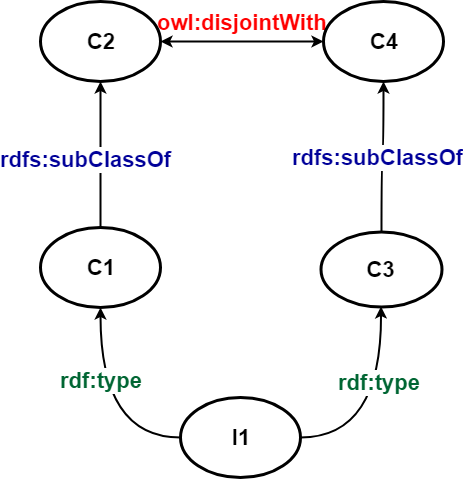
\includegraphics[width=0.5\textwidth]{images/Example1.png}
	}
	\subfloat[Example contradiction 2.\label{fig:Example2}]{%
		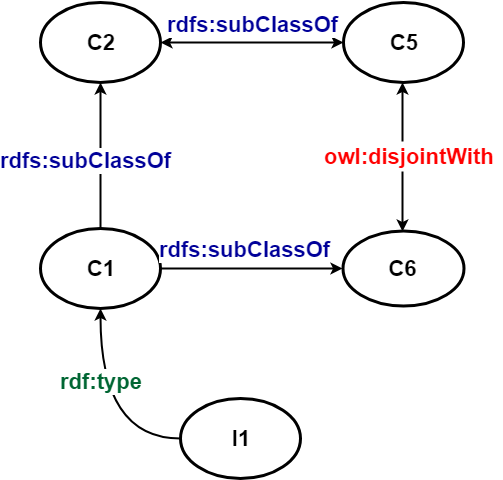
\includegraphics[width=0.5\textwidth]{images/Example2.png}
	}
	\caption{Showing 2 Examples to help understand the concepts we introduce in this work.}
	\label{fig:Antipattern}
\end{figure}

\textit{Example 1}. The first example\ref{fig:Example1} shows a simple contradiction, in this example we see an individual[I1], that is of two classes, for example "Monaco" is of type \textit{city in Europe}[C1] and of type \textit{country in Europe}[C3]. This is still correct, a instance can be of two different types. Now we define that a \textit{city in Europe} is a sub class of a \textit{City} and that a \textit{country in Europe} is a sub class of a \textit{Country}. This is still correct assumption. We now define that an \textit{City} can not be a \textit{Country} or the other way around by saying that a both classes can never have a individual in common. We now created an contradiction, as \textit{Monaco} is a individual of both, but it can not be.\\

Fixing this contradiction is possible, but it means that we need to change some things, we can either remove the disjoint axiom, meaning that now we can have a \textit{City} that is also a \textit{Country}. We could also split \textit{Monaco} into \textit{Monaco(City)} and \textit{Monaco(Country)}, which is also a possible solution. Both solutions have their positives and negatives, which need to be always taken into account.\\

\textit{Example 2}. The second example\ref{fig:Example2}, shows a different type of contradiction. This time we only have one rdf:type relation. This individual belongs to only one class, For example we have a individual \textit{}[I1] now is of the class \textit{ }[C1], This class has two subClass relations, with \textit{ }[C6] and \textit{ }[C2]. Where \textit{ }[C2] is also a sub class relation with \textit{ }[C5]. Which in turn is disjoint with \textit{ }[C6]. This makes the circle complete and generates another contradiction, as both \textit{ }[C5] and \textit{ }[C6] have an individual[I1] in common. \\


\section{Reasoner}
Now that we understand how the data is represented in knowledge graphs we can move on to the next part, reasoning. Reasoning is a method to find new information in the knowledge graph that was not explicitly written down. Reasoning comes in a multitude of flavours, but the two most common are deductive and inductive reasoning. 

\subsection{Reasoning types}
Reasoning is deriving facts from the ontology or knowledge base that has not yet been explicitly denoted. We can classify reasoning in several different subcategories, that are not a lot different from each other, but can have other optimized algorithms specialized in solving the different subcategories.

\begin{itemize}
	\item Satisfiability of a concept, determining if a description of a Class/Concept is not contradictory, As we shown in the examples, can we find an individual that satisfies the Class without creating a contradiction in the knowledge graph. 
	\item Subsumption of concepts, can we determine if a Class C is more general than Class D
	\item Consistency with respect to the ontology - determine whether individuals do not violate descriptions and statements that are described by the ontology.
	\item Check an individual - check whether the individual is an instance of a class
\end{itemize}

In this work we will focus on satifisfiability, but instead of finding the concepts that are satisfiable we will instead look for the opposite, and find the concepts and individuals that are unsatisfiable — thus finding if the knowledge graph is inconsistent, holding contradictory statements.

\textit{Inconsistency} An inconsistent knowledge graph is a graph that has one or more statements that are inconsistent with each other. A knowledge graph can have several types of inconsistency. It can be grammatically inconsistent. This happens when a statement is defined with the incorrect datatype. Here we focus on semantically inconsistency. This happens when a constraints that have been set by the language used in the knowledge graph have been broken. Shown in example \ref{} this happens when an instance is linked to two classes that are disjoint with each other. To find where a knowledge graph is inconsistent we use justifications.   

\textit{Justification}. A justification\cite{Horridge:2009} is a set of axioms that acts as an explanation for an entailment.
Formally, a justification is a minimal subset of the original axioms which are sufficient to prove the entailed formula. In this paper we interpret a justification as an explanation of contradiction. Given that our knowledge graphs are sets of triples, our justification are instantiated BPGs and are always minimal set of axioms for a single contradiction. \\


\section{Data}
We introduce four datasets that we use in this work, namely the pizza-ontology, DBpedia, YAGO, and LOD-a-lot.

\subsection{Pizza-ontology}
The first ontology we use in our work is the pizza ontology, it is developed by Manchester university. \cite{pizza}. The ontology describes pizza's and is used as an example ontology to explain how ontologies are created and how an ontology is used and expanded. The advantage of using this ontologies over others, or own made, is that this ontology is widely known, everyone can find this ontology on the web, and due to the ontology is a concrete example, we all know what a pizza is and what goes and does not go with a pizza. \\

\subsection{YAGO}
The final dataset we will use for experimentation is YAGO\cite{YAGO2:2013}, this dataset has derived 160 million statements from Wikipedia, WordNet and geoNames, about 10 million entities. This dataset is also made open source and is a joint project of the Max Planck Institute for Informatics and the Telecom ParisTech University. This dataset has great qualities for our experiments. The dataset has an temporal and special dimension, making it possibly prone to contradictions. The dataset is also manually evaluated and has according to \cite{YAGO2:2013} not a mistake free dataset, which is a good promise for our tests.

\subsection{DBpedia}
DBpedia\cite{DBpedia} is a crowd sourced project that extracts structural information from the Wikimedia, the foundation on which wikipedia, but also others, such as wikibooks, wikitionar, and wikidata belong. DBpedia is an ongoing project and at this moment their knowledge graph consists out of 1.8 billion statements about 4.58 million objects in the English version, and in total 9.5 billion statements if we combine all other languages as well. In this work we will focus on only the English version, as this has already been transformed to the correct fileformat for us. 

\subsection{LOD-a-lot}
The second dataset we use is the LOD-a-lot\cite{JavierD:2017} knowledge graph. The LOD-a-lot is created by Javier David Fernandez Garcia, Wouter Beek, Miguel A. Martínez-Prieto and Mario Arias, and holds more than 28 billion statements, from a collection of 600 thousand datasets. The size of this dataset of 28 billion triples and the heterogeneous datasets that have been used to create this knowledge graph make it great for contradiction retrieval. As the amount of different datasets could make it possible to find different sets of contradictions.

\newpage
\chapter{Related Work}\label{RelatedWork}
In this section an overview of work in various related research areas is provided. More specifically, we show the research on which this work is created on, the types of analyses that already have been implemented for knowledge graphs, and the techniques that show promise for sampling from knowledge graphs. \\

\section{Method}
Making a knowledge graph consistent has been an old problem, and solutions have been proposed since 1956 by Toulmin in his book \cite{toulmin:1956}, in which the solution is proposed by revising the base, choosing to reason only over the consistent subbases, expanded upon by Gabbay et al\cite{Gabbay:1994}. The second solution is to change the inference of the reasoner to fit the inconsistency, and can be seen as the first approaches to paraconsistent reasoning for example by Kaminski\cite{Kaminski:2015}.

With reasoning used in most software algorithms, the research done analysing inconsistent knowledge graphs has only been emerging in the last decade with the introduction of justifications by Horridge et al\cite{Horridge:2009}. In their paper the writers describe the framework used to retrieve the justifications from inconsistent knowledge graphs as minimal subsets of the graphs preserving the inconsistency. This forms an integral part of our algorithm. In the paper, they also explain why it is often time-consuming to retrieve all justifications for ontologies. In the paper by T\"{o}pper et al. \cite{Topper:2012} they, propose a solution to identify contradictions in DBpedia, with handcrafted `anti-patterns'. With the extraction of `anti-patterns' from the Lod-a-lot we have a generalised approach that works on any knowledge graph. \\


Previous work locating contradictions has been done by \cite{Eiter:2010} 
McAreavey expanded upon the notion of contradiction by ...
\cite{McAreavey:2014}

Finally Zhi et al. Did this:
\cite{Zhi:2015}

But our method is better.


Our method re uses part of the method that has been developed by Azad Noori et al\cite{Noori:2015}. In this paper they propose an efficient algorithm for pathfinding that we use in our subgraph generation and in our sampling.

\section{Analysis}
Paulheim \cite{HeikoP:2016} showcases the need for a standardised evaluation method. In the survey, they show that researchers sometimes choose different knowledge graph(s) according to their needs, this makes it harder to compare different algorithms. Removing this discrepancy would benefit all of us.

F\'arber et al. \cite{MichaelF:2017} give an in-depth comparison of several large knowledge graphs, and demonstrates that knowledge graphs hold different metrics. The paper by F\"arber et al. \cite{MichaelF:2017} is expanded upon by Debattista et al. in \cite{Debattista:2018}, in which they analysed 130 datasets from the Linked Open Data Cloud using 27 Linked Data quality metrics. Both papers show that each graph has a different underlying structure and in theory, this even can result in different behaviour of algorithms.

The paper by Peter Bloem and Steven de Rooij\cite{BloemP:2018} would be a good usecase in which we could implement our anti-patterns for analysis. With an combination of implementations we couldmake statistical inferences about if `anti-patterns' occur with regularity. Which would incredibly useful for making automatic software for contradiction detection.

\section{Sampling}
In the paper by Jure Leskovec and Christos Faloutsos \cite{Leskovec:2006} several sampling techniques are proposed and compared, and with it they show that even naive sampling such as random walks and 'forest fire' show accurate results, even sampling to 15\% of the original size. 
\cite{Jin:2011} Albatross sampling, shows a sampling technique designed for loosely connected or disconnected networks, especially for social networks, while
This technique could be useful for sampling graph networks, as the algorithm gives an even more accurate sample, but due to an extra constraint we've put on with the justifications, this sampling technique could not be applied.

In the paper by Kurant et al.\cite{Kurant:2011}  are explaining the bias that forms when implementing breath first sampling.
While this paper has no direct effect on the implementation the information described in the paper is useful to explain why our samples have some discrepancies when it comes to the differences in indegree and outdegree. 

Finally Rietveld et al.\cite{Rietveld:2014} shows that sampling for targeted use, in their case SPARQL coverage is possible, this shows that sampling a knowledge base, for targeted cases can generally be relevant for multiple reasons.

\newpage

\chapter{Defining the problem}\label{ProblemDefintion}
In the last chapter we introduced the related work we used in this work as a basis for the method we introduce in the method. In this section we introduce a formal approach to the problem we introduced in the introduction. The problem formalization crucial in the aim of this work in order to understand the method we propose in the next section.

\section{Problem Description}
At the moment most large knowledge graph have contradictions, but with reasoners only being able to reason on smaller knowledge graphs, we do not know much about the composition of the contradictions in the knowledge graphs. Understanding how the contradictions have formed, or where the contradictions occur, is crucial information when we want to develop better tools that can handle larger knowledge graphs. The second problem is that, while implementing solutions on a large scale is preferable, testing and benchmarking on smaller knowledge graphs that match existing knowledge graphs would be more accurate. As natural knowledge graphs and that have known properties and contradictions instead of synthesised knowledge graphs is preferable. 

To solve the issues, we split it into three parts. The first part is to locate the contradictions within the knowledge graph. Only contradictions that are known can be treated as such, as sampling later in the pipeline can only work with contradictions that are known beforehand to sample accordingly.
The second part of the problem is the knowledge graph analysis. Analysing the graph gives useful statistics about the knowledge graph, and helps us understand the knowledge graph also with respect to the found inconsistencies in the first part.

The final part of the problem is the sampling of the knowledge graph. Is it even possible to sample from the original knowledge base and keep the characteristics we measured in the second part of the problem on the same level as the original large knowledge graph? Moreover, can we make sure that the sampled graph still holds the number of inconsistencies we want the graph to have? 

\subsection{Research questions}
To formalize the problem description, the following research questions are formulated.
\begin{itemize}
	\item \textbf{RQ1}: Can we describe and define a formal definition for general contradiction patterns, where general contradiction patterns are inconsistent subgraphs which are persistent throughout all natural knowledge graphs?
	\item \textbf{RQ2}: How can we retrieve the general contradiction patterns that have occurred in natural knowledge graphs? 
	\item \textbf{RQ3}: What classifications are there which can classify groups of general contradiction patterns? And what main characteristics can describe the classes of contradiction patterns best? Can we use these commonalities to give better qualitative and quantitative information about the graph?
	\item \textbf{RQ4}: Are there methods, or can we design methods that could benefit from using general contradiction patterns in their algorithm? 
	\begin{itemize}
		\item Are we able to improve analytics about contradictions for large linked datasets, by giving qualitative and quantitative information about a linked datasets?
		\item Can we use the anti-patterns, to build benchmarks. Benchmarks that have been sampled from large, but inconsistent datasets with general contradiction patterns. Would it be possible to keep the sampled characteristics invariant from sampling?
	\end{itemize}
\end{itemize}

\section{Anti-pattern definition}
 We already explained the term  `anti-pattern' a bit in the introduction, but in this chapter we will introduce the term officially, and come to a definition of what a `anti-pattern' exactly is, and how we can derive `anti-patterns' from sets contradictions. \\

To understand how an `anti-pattern' is formed we first need to understand what a contradiction is. As shown in the examples we see a logical contradiction, with it we mean that a there is a logical mismatch between to rules that force the model to be inconsistent. Either one rule is true, in the first example it could be that the rule is `rdfs:subClassOf' between Class C1 and C2 is true, but then the rule `owl:disjointWith' should not be there. Or it can be the other way around, the rule `rdfs:subClassOf' is removed and only the rule `owl:disjointWith' exists. But it can not be that both rules exist, as this creates an contradiction. \\

The second example shows we can a similar contradiction. In the second example we find two different contradictions, the first ... and the second... What is noticable is that in this example we can proof a contradiction in two seperate ways, while using some of the same axioms. \\

As explained in chapter \ref{graphElements} a justification is a description of a single contradiction, we can see it as a proof that an ontology is inconsistent. Each justification is an instantiated BGP, within the knowledge graph. Due to the instantiation, the justification can only describe one contradiction, and is thus limited to a single knowledge graph. To use justifications in other knowledge graphs, to check if this knowledge graph has the same contradiction, without having the same information, we need to generalize the justification. If for example we have a knowledge graph describing the contradictions in the knowledge graph of Countries in Europe, wherein we wrongfully declared Monaco a city and a country, without the consideration that they are disjoint. we want to quickly check if the same has happened for our knowledge graph from Asia. Without a generalisation, we first need to check if what relations are in the knowledge graph in Asia, and if there is a city matching the particulars.\\

For generalization we created `anti-patterns'. `Anti-patterns' are generalisations over justifications, to transform an justification into an `anti-pattern' we remove all information on the subject and object position of the BGP. Removing the information on the predicate position("owl:disjointWith", "rdfs:subclassOf", "rdf:type", etc) would break the contradiction, as it it would be possible to match a "rdfs:subClassOf" on the place where the "owl:disjointWith" belongs. This would make the contradiction no longer a contradiction.  
Now that we removed all the information that blocks generalization, we are left with the `anti-pattern'. Now the `anti-pattern' can be used to match various inconsistent justifications in the knowledge graph. We define an \textit{`Anti-pattern'} in the following definition:\\

\begin{definition} 
	An \textit{`Anti-pattern'} \textit{of a knowledge graph G is a minimal set of uninstantiated Basic Triple Patterns that match an inconsistent subgraph of G.}
\end{definition}

We show the conversion of a justification(instantiated BPG) to an `Anti pattern' (uninstantiated BPG) in figure \ref{fig:JustificationtoGeneral}.


\section{Plan of attack}
The first step before we can do any analysis is to retrieve the `anti-patterns'. The method we developed is not based on any work that has been previously created, instead we opted to develop our own method. The method is designed specifically to retrieve `anti-patterns' from large knowledge graphs. Which are generalised contradictions, and can be seen as common mistakes made in dataset. We described a formal notion of `anti-patterns' in chapter \ref{AntiPatternDefinition}. Our method for retrieval is a three stage pipeline, the results of the previous stage flow into the next stage. With the input being a knowledge graph, in our case this is the LOD-a-lot\cite{JavierD:2017} a dataset containing 28 billion statements. The output from the final stage will be the found `anti-patterns'. 

\subsection{Proposed Applications}
With the `Anti-patterns' found we we developed two implementations that benefit greatly from `anti-patterns', The first being analysis for inconsistent knowledge graphs and the second a sampling method which uses `anti-pattern' in its sampling. The first implementation, analysis takes any arbitrary knowledge graph and analysis this graph on the basis of the found `anti-patterns'. Which helps us understand what types of `anti-patterns' occur in a knowledge graph, giving us a better overview of inconsistent knowledge graphs in general, answering our second research question.

The second implementation, sampling is a common use case for other research topics as well. The reason for this implementation is that benchmarking for a number of research topics, such .... all use knowledge graphs that have been specifically designed for testing, such as ... and  .... . While this could work for testing, it could be that algorithms perform not as well on natural knowledge graphs. But due to the size of natural knowledge graphs, such as YAGO, DBpedia, and LOD-a-lot, it will be time-consuming to test on these knowledge graphs without knowing if the algorithm even works. To combat this sampling can be used to retrieve a smaller part of the knowledge graph we want to test on and use this sample to test the algorithm on. While sampling is a good practice to shrink the testspace, it could be that the sample lost some of the characteristics of the original knowledge graph. 

We designed a different sampling technique that uses `anti-patterns' as a basis for sampling, this sampling technique uses the found `anti-patterns' to build a knowledge graph that is inconsistent, with respect to the original knowledge graphs. Secondly the sampling can be used to sample a knowledge graph that only has a set of specific `anti-patterns'.

\subsection{Proposed Experiments}
Now that we set up our method, we show the how this method performs by three experiments. 
Firstly we test if we can retrieve `all' justifications from the knowledge graph, due to the extraction process in the pipeline we can not guarantee that we can extract every contradiction from the knowledge graph. Which means that it is possible for the method to miss contradictions, and thus it can be possible that we miss the accompanying `anti-patterns' that we could have derived from the contradictions. To test this hypothesis that we can retrieve most to all `anti-patterns' we developed a experiment by extracting all the contradictions from the pizza-ontology. We choose this ontology as it is a simple to use ontology with concrete statements that are understood by everyone. It makes it simple to check by hand if the amount of `anti-patterns we found, matches the amount of `anti-patterns' we found with our extraction method.

Secondly we test if we can analyze knowledge graphs, we have two inconsistent knowledge graphs, DBpedia and YAGO, both with known contradictions. We retrieve the statistics about the knowledge graph. We then retrieve all the `anti-patterns' that have instantiated contradictions in the knowledge graph. 
With this experiment we want to show the use of `anti-patterns' to get a better understanding of how inconsistent knowledge graphs are formed, and what types of `anti-patterns' are more common than others.

Thirdly we test if we can sample a set of inconsistent knowledge graphs. We examine this by experimenting with a set of large knowledge graphs and test if we have replicated the original knowledge graph in a smaller variant, as well as a measure if the number of contradictions matches the number of contradictions we have set.

\newpage
\chapter{Finding `Anti-patterns'}\label{Method}
\begin{figure}[!t]
	\centering
	\makebox[\textwidth][c]{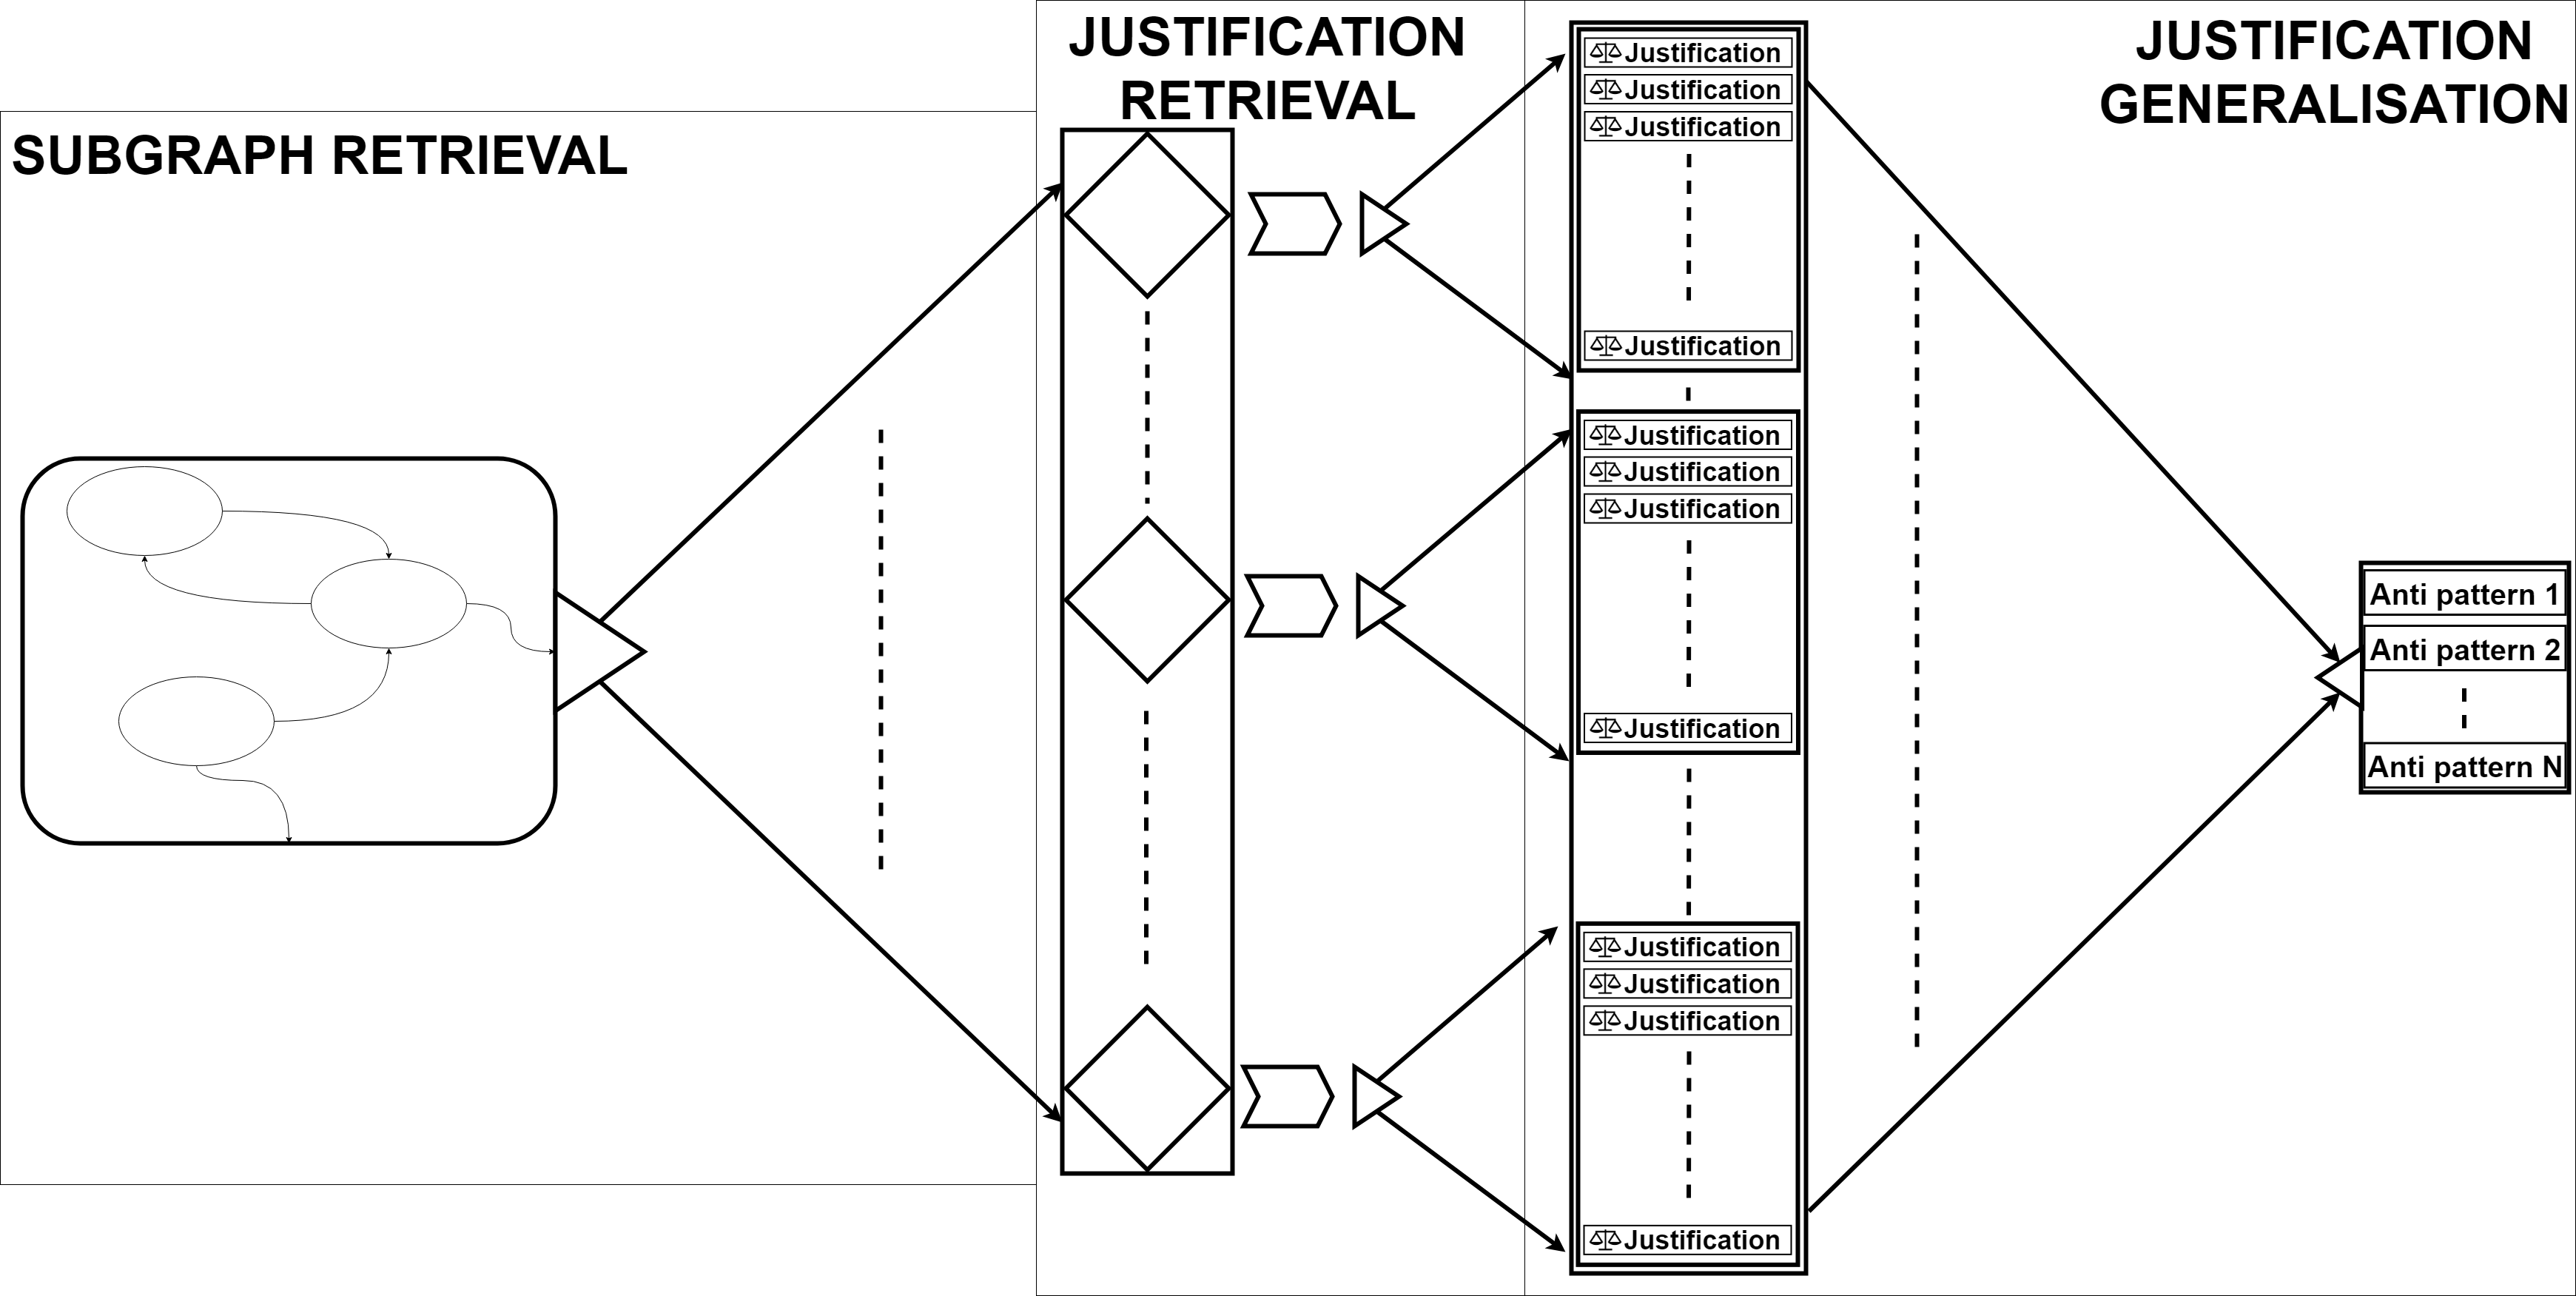
\includegraphics[width=0.8\textwidth]{images/SimplifiedPipelineMissingPart.png}}
	\caption{A schematic diagram that shows the pipeline used to extract subgraphs, find justifications and their `anti-patterns'. Finally 
		we use the information that we retrieved, to analyse and sample the Knowledge graph.}
	\label{fig:simplePipeline}
\end{figure}
Our extraction method consists of three aspects: Firstly, we retrieve smaller subgraphs from the knowledge graph from which we want the contradictions. Secondly, from each subgraph, we check if the graph is inconsistent and retrieve the justifications. Finally, with the justifications, we create the `anti-patterns'. The entire pipeline is shown in figure \ref{fig:simplePipeline}.\\
Our pipeline is designed to find `almost' all the `anti-patterns' in any knowledge graph. We implemented techniques to find these smaller inconsistent subgraphs with OWLAPI\cite{Horridge:2011} and Openllet\cite{Openllet:2019} which based on work of Pellet\cite{Pellet:2007}.\\

\section{Algorithmic overview and proof}
We can prove that the algorithm can retrieve all `anti-patterns' from a given knowledge graph. We start by stating that it is possible to retrieve all inconsistency justifications in a knowledge graph, as has been proven by \cite{Horridge:2009}. Lets assume that we retrieved all justifications from a knowledge graph. We can know that also retrieved all `anti-patterns'. Each `anti-pattern' has one or more justifications that is contained in the knowledge graph. \\

\begin{algorithm}[H]
	\KwData{The knowledge graph that holds contradictions we want to extract}
	\KwResult{the set of `anti-patterns' found in the knowledge graph}
	
	retrieve all justifications in the knowledge graph\\
	\ForEach{justification in list of justifications}{
	convert `anti-pattern' from justification\\
		\eIf{`anti-pattern' is not known}{
			add `anti-pattern' to list of known `anti-patterns'
		}{
			skip `anti-pattern' as we already know it.
		}
	}
\Return list of `anti-patterns'\\
	\caption{Algorithmic view of the method}
\end{algorithm}

\section{Subgraph retrieval}
\begin{figure}[!t]
	\subfloat[A diagram that shows the retrieval and splitting of subgraphs from the knowledge graph.\label{fig:subgraphRetrieval}]{%
		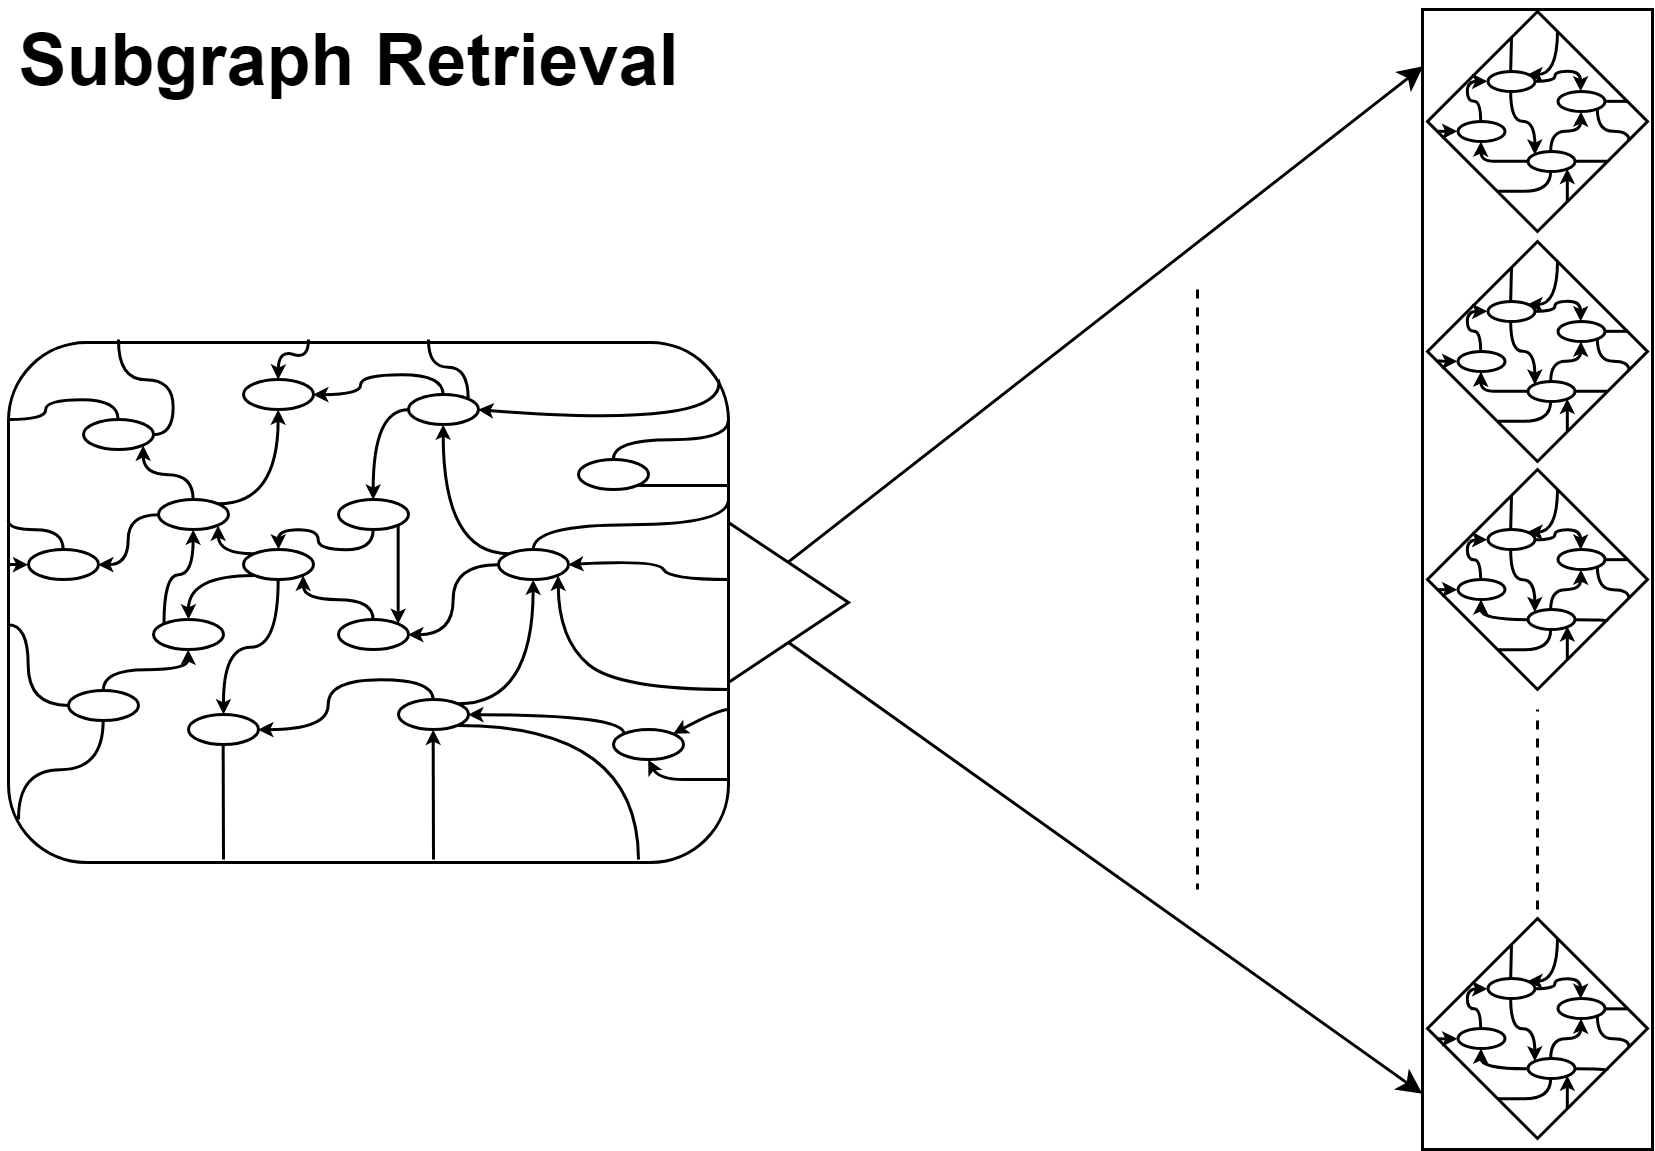
\includegraphics[width=0.45\textwidth]{images/SubgraphRetrieval.png}
	}
	\hfill
	\subfloat[A diagram that shows the retrieval of justifications from a single subgraph.\label{fig:JustificationRetrieval}]{%
		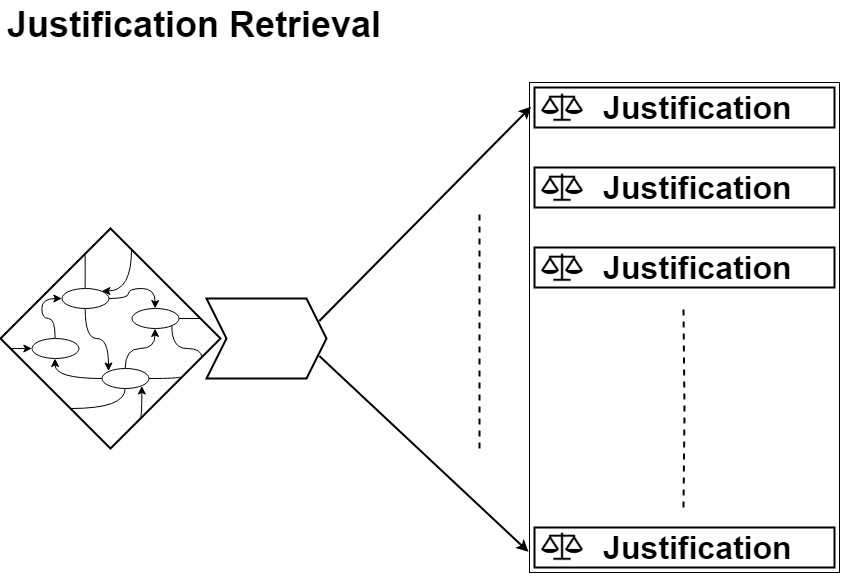
\includegraphics[width=0.45\textwidth]{images/JustificationRetrieval.png}
	}
	\caption{zoomed in diagrams of the first part of the pipeline}
	\label{fig:PipelinePart12}
\end{figure}
Due to the large size of most knowledge graphs, running a justification retrieval algorithm over the complete knowledge graph, to retrieve all contradictions would be impractical. To speed up this process, we decided to split the knowledge graph into smaller chunks to reduce the time the justification retrieval algorithm needs to find all justifications in the smaller subgraphs. Figure \ref{fig:subgraphRetrieval} shows the process of splitting the knowledge graph into smaller subgraphs.
Each subgraph is generated by extending the root node. The root node is retrieved by taking a triple from the complete graph and taking the node that is in the subject position as the starting point. The graph is expanded by finding all the triples that have the root node as the subject, and we add these triples to the subgraph. Next, all the nodes that were in the object position are now used as expansion nodes, so now for each object, we now find all the triples that match where the object is put in the subject position. We keep expanding the graph until it can not expand any further or the maximum amount of triples of 5000 triples is reached. The value of 5000 triples is chosen because it is large enough to hold almost all justification patterns but small enough that it does not take long to retrieve all justifications.\\
While this method to sample subgraphs from the knowledge graph does not guarantee completeness in terms of finding all the contradictions that can occur, but we show that this method finds the `almost' all occurring contradictions, with the help of redundancy, without occurring too many time-consuming calculations. 

\section{Justification retrieval}
With the knowledge graph split into smaller chunks, we can now move on the next step in the extraction pipeline, as shown in figure \ref{fig:JustificationRetrieval}.
With the newly formed subgraphs, we start with the check if the graph is consistent or inconsistent. If the graph is consistent, we can skip this graph, as the amount of contradictions is zero.\\ 
If the graph is inconsistent, then we find the reason or reasons why, a graph can be inconsistent due to a single contradiction, or it can have multiple contradictions. 
To find all the contradictions we use the justifications algorithm in the Openllet reasoner. The justifications algorithm walks through the graph and finds the minimal justification for each contradiction. The algorithm continues to search for justifications until no more justification can be found in the graph. This is done for each subgraph, and all the justifications are then pushed through the extraction pipeline to the next stage.\\

\section{Justification generalization to `anti-patterns'}
While all justifications are different as each justification is a set of instantiated BTP, the underlying uninstantiated BGP does not have to be. The underlying BGP forms the basis of the `anti-patterns'. The `anti-patterns' describe a set of contradictions, that has been found in the inconsistent knowledge graph. The `anti-patterns' can be used to locate inconsistencies in other knowledge graphs as well. In Figure \ref{fig:PatternGeneralizing} we show the last part of the pipeline, the conversion of all justifications to a set of `anti-patterns'.

\begin{figure}[!t]
	\subfloat[A schematic diagram showcasing how the justifications are transformed into Generalized inconsistency patterns.\label{fig:PatternGeneralizing}]{%
		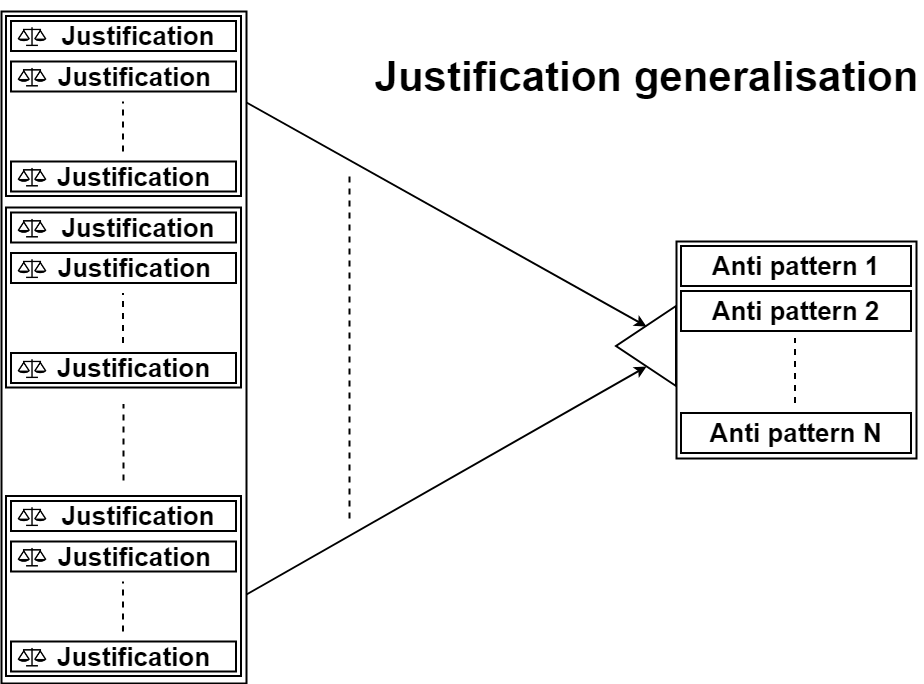
\includegraphics[width=0.45\textwidth]{images/PatternGeneralizing.png}
	}
	\hfill
	\subfloat[A diagram that shows the transformation from Justification to a `anti-pattern'.\label{fig:JustificationtoGeneral}]{%
		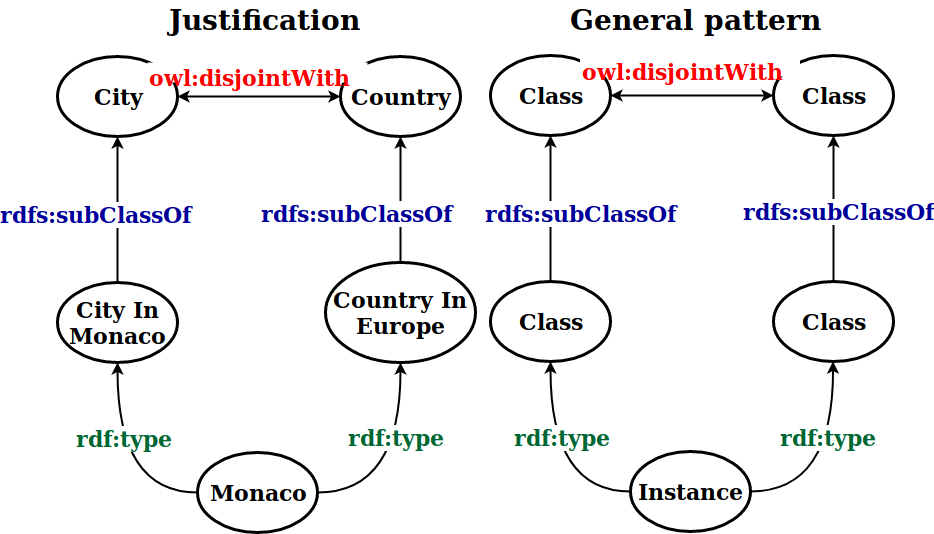
\includegraphics[width=0.45\textwidth]{images/JustificationtoGeneral.png}
	}
	\caption{zoomed in the diagram of the third part of the pipeline, as well as a closer look into justifications and general graphs.}
	\label{fig:PipelinePart3}
\end{figure}
To get the `anti-pattern' from the justification, we first generalise the justification by removing the instantiated subject and object on the nodes as shown in figure \ref{fig:JustificationtoGeneral}. This gives the possibility to generalise the justification purely on its structure instead of its instantiated subject and object. While the informat
ion in the nodes is not essential, the information on the edges is. Graphs with different edges can be seen as different contradictions. \\
If we, for example, change the `owl:disjointWith' into `rdfs:subclassOf' and transform one of the `rdfs:subclassOf' into an `owl:disjointWith' We have a different inconsistency pattern. For this reason, we need to store the edges in the `anti-pattern'.\\
With the justifications now devoid of information on the nodes we now group the justifications per `anti-pattern'. This means that each justification that has the same underlying `anti-pattern' is isomorphic, even with respect to the edges in the pattern. \\
To find these isomorphisms we have implemented a version of the VF2 algorithm\cite{LCordella:2004}, with the addition to the algorithm that we also match the edges of the two justifications. Checking if two graphs are not isomorphic is NP-intermediate. Therefore we added in additional heuristics that need to match first before we apply the VF2 algorithm. Firstly we check if a graph has the same number of vertices, the same number of edges, the same amount of degrees, and in our case it also needs to have the same amount of edges based on the edge types we have. If all these matches then we apply the VF2 algorithm to the two `anti-patterns'. If the algorithm matches a justification to the found `anti-patterns', it adds this particular justification to this `anti-patterns', but if no pattern can be matched to the justification, a new `anti-patterns' is formed from this justification. This algorithm continues until all patterns have been matched to their correct `anti-pattern' group.\\

\section{Design decisions}
To speed up the process for finding all `anti-patterns' in large knowledge graphs we made design decisions that do longer guarentee that we can find all `anti-patterns'. We need to take these design decisions as it would else be intractable to go locate all `anti-patterns' as the algorithm would take too long to finish. 
The first decision is to split the knowledge graph into smaller subgraphs. This makes it possible to for the reasoner to quickly check if the subgraph is consistent and retrieve all `anti-patterns' from the subgraph. To make sure we still find each `anti-pattern' we overlap the subgraphs such that it is improbable that we miss an contradiction, because it was split and put into two different subgraphs.\\
The second design decision is that we put in a cut off into the amount of justifications the reasoner can find in the subgraph. We put this cut off in there deliberately. The reasoner, Openllet can continue indefinitely to find new justifications in a graph if no cut off is given \cite{Openllet:2019}. So this was one of the contraints that we needed to implement due to the chosen reasoner. 
The final algorithm is shown in image \ref{finalAlgorithm}.\\
\\
\begin{algorithm}[H]
	\KwData{The knowledge graph that holds contradictions we want to extract}
	\KwResult{the set of `anti-patterns' found in the knowledge graph}
	KnowledgeSubgraphs split(knowledge graph)\\
	
	\ForEach{subgraph \textbf{in} KnowledgeSubgraphs }{
		retrieve all contradictions in the subgraph\\
		\ForEach{contradiction in list of contradictions}{
			convert `anti-pattern' from contradiction\\
			\eIf{`anti-pattern' is not known}{
				add `anti-pattern' to list of known `anti-patterns'
			}{
				skip `anti-pattern' as we already know it.
			}
		}
	}
	\Return list of `anti-patterns'\\
	\caption{Algorithmic view of the method}
	\label{finalAlgorithm}
\end{algorithm}

\newpage
\chapter{Testing the pipeline}\label{Experiments}
In the following sections we describe the experimental setup, this subsection explains which experiments we performed, how the system around the experiments is set up. We will then explain each individual experiment per subsection. In total we will show 2 experiments that show the `anti-patterns' we retrieved from the LOD-a-lot, and we will analyze the results from the experiments. 

\section{Experimental Setup}
\textit{Datasets}. In the section background we already described the datasets we used for our experiments. We use the pizza ontology in the first experiment to showcase how we retrieve the `anti-patterns' from knowledge graphs. In the second experiment we show the retrieved `anti-patterns' from the LOD-a-lot.

\textit{Method and Implementation software}. Both the method and the implementations, which we will explain in section \ref{Implementation} have been written in JAVA. We choose JAVA as the programming language for the amount of libraries that have been made available in JAVA. The the most important libraries we used for the implementation are, jena, rdf2hdt, openllet and OWLapi, all available as open source. It is noted that the retrieval of the `anti-patterns' has been done on the LOD server, due to the time it took to retrieve the `anti-patterns' from the LOD-a-lot. 

\section{Experiment 1: \textbf{RQ1}:  Can we design a pipeline that can retrieve a (sub-)set inconsistencies and translate the inconsistencies to `anti-patterns'?[Completeness]}
% Describe how the creation of the inconsistencies from the lod cloud worked.
\textit{Experiment description}. The purpose of this experiment is to show that we can indeed extract inconsistencies from an arbitrary knowledge graph, with the pipeline. 
To show that the pipeline works we have tested the algorithm on two extreme cases — the first case being the pizza ontology and the second case the LOD-a-lot.
The pizza knowledge graph is great for measuring the completeness of the inconsistencies found and shows it is measurable if the reasoner can find the different inconsistencies. Which can be easily checked by hand.\\
Because we can not prove that our pipeline guarantees the completeness, we test if the pipeline still retrieves all `anti-patterns' even when the size of the subgraph is 
smaller than the size of the knowledge graph.\\
\textit{analysis}. We compare the results of our method for retrieving the `anti-patterns' from the pizza ontology with the contradictions found by the reasoners in prot\'{e}g\'{e}.
The results are summarized in Table \ref{table:GraphStats}. The first column shows the size of triple subgraphs we used, In the first part of the algorithm we split the knowledge graph into smaller subgraphs, this size can be adjusted to improve speed vs redundant triples. In this table we show that even with smaller subgraph sizes our algorithm still retrieves the same `anti-patterns' as the reasoners. The `anti-patterns' found by the reasoners are contradictions which are then transformed by hand to `anti-patterns'. 

\begin{table}[!t]
	\centering
	\makebox[\textwidth]{
		\begin{tabular}{|l|l|l|}
			\hline
			& Inconsistent? & Found inconsistencies \\ \hline \hline
			250 triple subgraphs     & Yes           & 9\\ \hline
			500 triple subgraphs     & Yes           & 9\\ \hline
			1,000 triple subgraphs     & Yes           & 9\\ \hline
			5,000 triple subgraphs     & Yes           & 9\\ \hline
			Pellet                     & Yes           & 6\\ \hline
			HermiT                     & Yes           & 6\\ \hline
			Pellet                     & Yes           & 6\\ \hline
	\end{tabular}}
	\caption{table showing the reasoners to test the pizza ontology.}
	\label{table:PizzaOntology}
\end{table}

\section{Experiment 2: \textbf{RQ1}:  Can we retrieve `Anti-patterns' more efficiently with splitting or not?[Efficiency]}
% Describe how the creation of the inconsistencies from the lod cloud worked.

\section{Experiment 3: Anti-pattern Analysis} % Renaming
\textit{Experiment description}. 

\textit{Retrieval} The second experiment shows the retrieval of the `anti-patterns' from the LOD-a-lot. We posted all the `anti-patterns' found on the website \url{https://thomasdegroot18.github.io/kbgenerator/}. On this website we generate the SPARQL queries for every `anti-pattern' and we show an visualization of the found `anti-patterns'.  

\textit{Analysis} In the images ... and ... We show examples of the `anti-patterns' we found. We found that we can split the `anti-patterns' into four groups. The first group is are simple circles with with only two \textit{rdf:type}, \textit{rdfs:subClassOf} and \textit{owl:disjointWith}. The second group is a circle with an attachment. There is only one isntance with \textit{rdf:type}. Then there are several \textit{rdfs:subClassOf} and one \textit{owl:disjointWith} relations. The third group is equal to the first group circle, but with the addition of \textit{owl:equivalentWith}. The fourth group is equal to the second group, but also with one or multiple \textit{owl:equivalentWith}. \\

Each group has several distinct features 

\newpage
\chapter{Applications for `anti-patterns'}\label{Implementation}
As shown in figure \ref{fig:PipelinePart45} we show the two implementations that make use of `anti-patterns' that we can findwith the previous section. The first implementation is the use case of analysing the knowledge graph in its entirety, as well as looking at how the inconsistencies occur within the larger knowledge graph. We use the analytics of the knowledge graph later in the sampling implementation. Secondly, we showcase that the sampling technique, with respect to the found `anti-patterns' in the graph that we used, produces similar albeit smaller knowledge graphs.

\section{Analysis tool kit for inconsistent knowledge graphs}
In this paper, we show the implementation of analysing knowledge graphs on a range of characteristics. Our analysis of the knowledge graphs is split into two aspects. The first part is the retrieval of general statistics about the knowledge base:
\begin{itemize}
	\item The number of triples of the knowledge graph.
	\item The Expressivity of the logic language that is used in KB.
	\item The number of distinct namespaces in the knowledge graph.
	\item The number of distinct predicates used in the knowledge graph.
	\item The distribution of indegree over all the nodes.
	\item The distribution of outdegree over all the nodes.
	\item The distribution of the Clustering Coefficient over all the nodes in the graph.
\end{itemize}

The second part of the analysis is specifically aimed at inconsistency statistics. We locate all contradictions that match the `anti-patterns' that have been found by retrieving `almost' all `anti-patterns' from the LOD-a-lot. With the `anti-patterns' we can retrieve the needed statistics that characterise the knowledge graph. The metrics that we use in our analysis are:
\begin{itemize}
	\item Amount of `anti-patterns' in the knowledge graph.
	\item Largest `anti-patterns' by a number of basic triple patterns found in the knowledge graph.
	\item Distribution of the occurrences of contradictions found in the knowledge graph.
	\item Distribution of the sizes of `anti-patterns' found in the knowledge graph.
\end{itemize} 

\begin{figure}[!t]
	\subfloat[This diagram shows one of the usecases for the `anti-patterns', namely Analytics.\label{fig:AnalyticsDrawing}]{%
		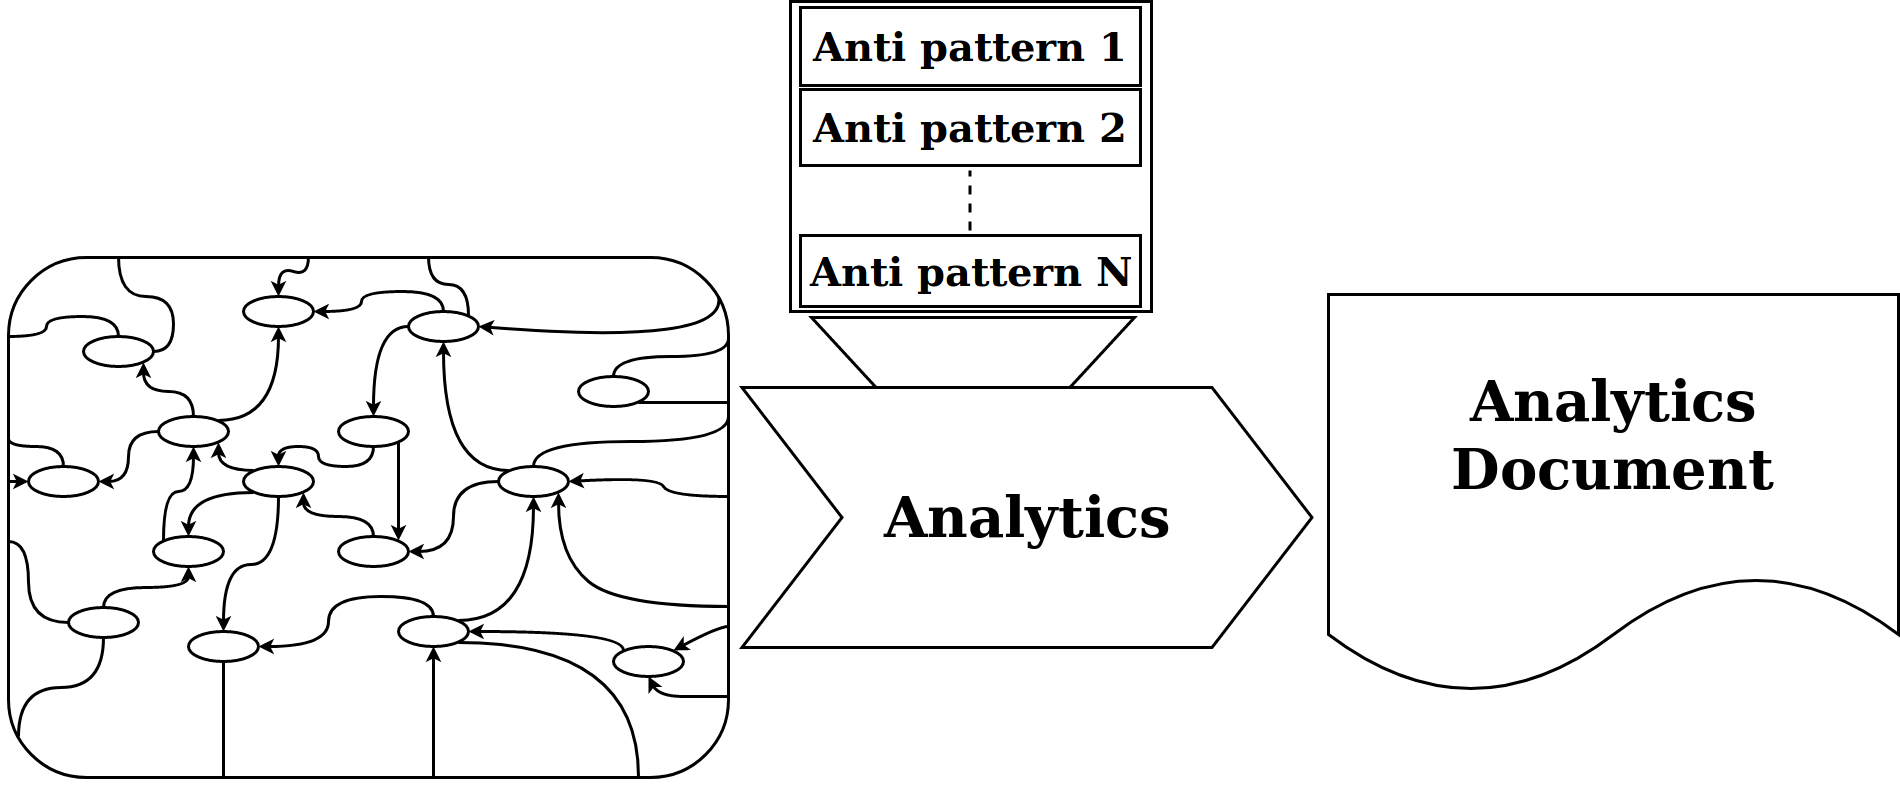
\includegraphics[width=0.45\textwidth]{images/AnalyticsDrawing.png}
	}
	\hfill
	\subfloat[This diagram shows the second usecase for the `anti-patterns', Sampling.\label{fig:SamplingDrawing}]{%
		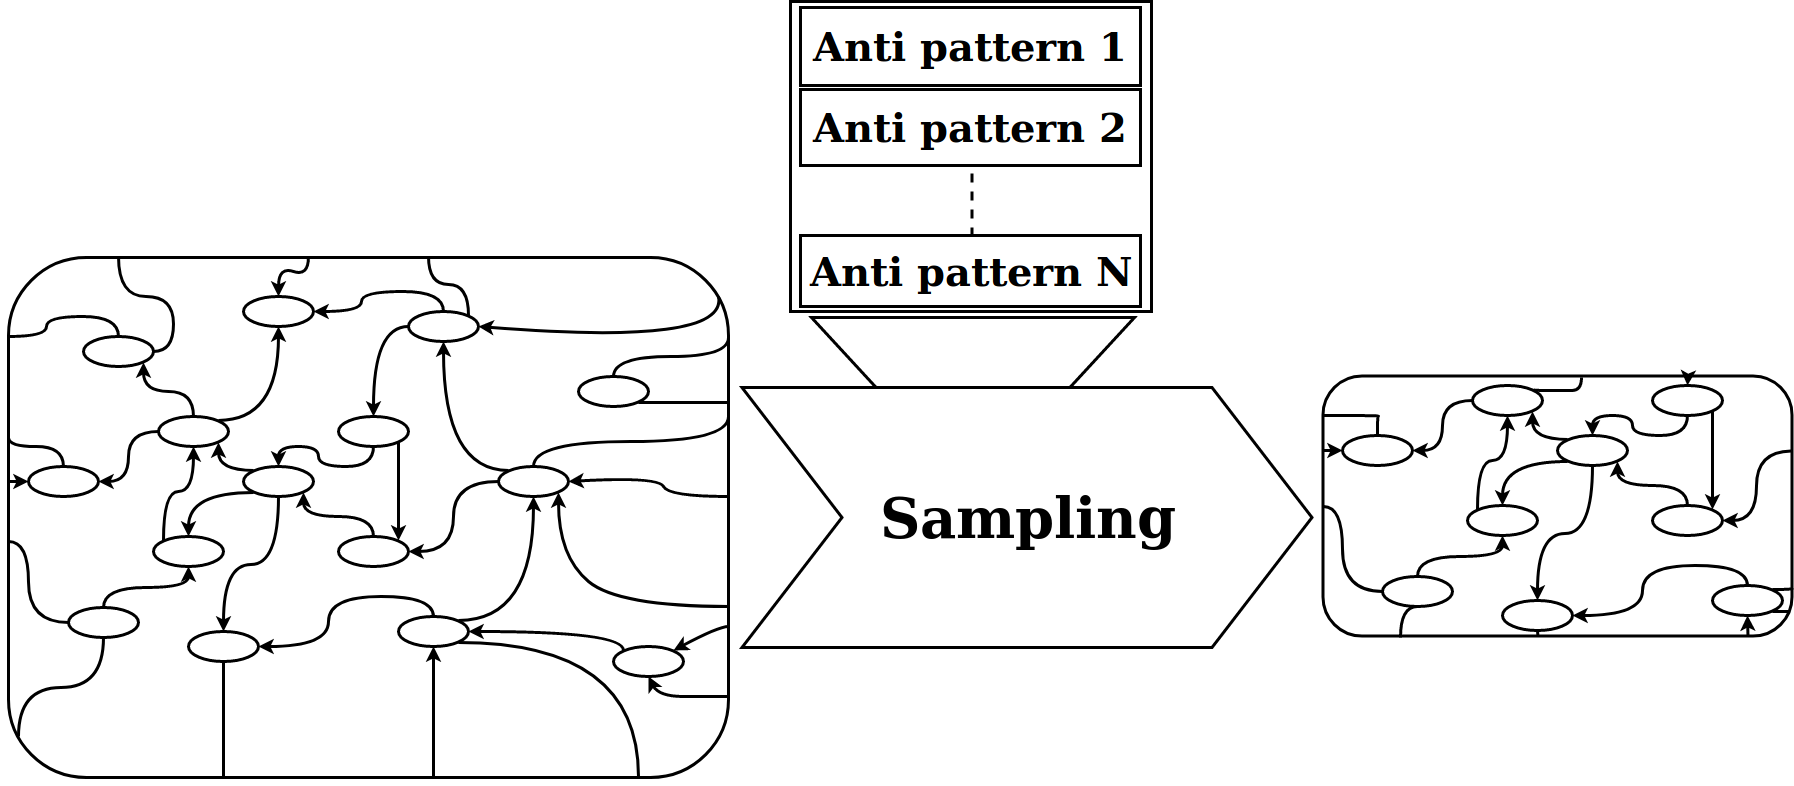
\includegraphics[width=0.45\textwidth]{images/SamplingDrawing.png}
	}
	\caption{zoomed in diagram of the final parts of the pipelines.}
	\label{fig:PipelinePart45}
\end{figure}

\section{Sampling tool kit for inconsistent knowledge graphs}
The second implementation that makes use of the `anti-patterns' is the implementation of sampling a knowledge graph. In this paper, the goal of sampling is to sample a knowledge graph into a smaller partition with two constraints. the first constraint is that, we make sure that the knowledge graph stays connected. Secondly, we give the user the possibility to choose the `anti-patterns' and the minimal amount of contradictions that can be in the sample.
To achieve the goal of sampling while keeping the constraints in mind means that we can not use any techniques that start from a node,, or a set of nodes, such as random walks, or forest fire sampling. Because we then cannot guarantee connectedness or the minimal amount of contradictions.\\ 
Our algorithm instead uses random constrained deletion; this algorithm randomly deletes triples that can be safely deleted. Triples that are connected to contradictions, or hold the only connection between subgraphs cannot be deleted.
The first set of triples that can not be deleted are the triples that describe the contradictions. To make sure that contradictions are not deleted, we start by building an HDT\cite{FMPGPA:13}\cite{MPAF:12} that stores all the triples that make up these contradictions. We use a SPARQL query to find the results of each of the `anti-patterns', and retrieve the number of contradictions the user wanted as BTPs. The triples are then combined and converted to an HDT. The algorithm can now check if a triple can be safely deleted. By checking if the triple is not present in the HDT.\\
The second set of triples that can not be deleted are the triples that break the to sample graph into smaller subgraphs. To negate this problem the algorithm uses local connectedness. A triple may only be safely deleted if there is a second path that connects the object and the subject without having to pass through the severed link. There is one exception to the rule when either the subject or the object does not have any other links, the triple is then is also allowed to be deleted. With this, we can guarantee that the graph does not split into smaller subgraphs. \\%TODO: Can we guarantee local connectedness?
The sampling by random deletion now continues to delete triples until the sample reaches the size given by the user, or when it is no longer able to delete triples. This can happen either because the only triples that can be deleted split the graph into subgraphs, or the only triples that can be safely deleted belong to the non-deletable contradictions.

\newpage
\chapter{Application Experiments}
Next we will show the results of the two implementations we designed, which we will also analyze. In these experiment we use YAGO, and DBpedia for analysis and sampling, as well as the `anti-patterns' from the LOD-a-lot as the `anti-pattern' input. With the expectation that the `anti-patterns' from the LOD-a-lot will encompass all the `anti-patterns' from the to sample datasets.\\


\section{Experiment 4: \textbf{RQ3}: Implementation 1, Analysing inconsistent graphs}
\textit{Experiment description}. We retrieved the statistics from several knowledge graphs differing in size. This implementation of knowledge graph analysis a typical showcase. In this experiment we retrieve relevant statistics from YAGO, DBpedia knowledge graphs and ... as we explained in section \ref{Implementation}.   \\

\textit{Analysis}. Table \ref{table:GraphStats} shows the analytics about the knowledge graph. As noticed the results show several distinctions between the three different knowledge graphs. Even though their expressiveness and the size do roughly match their number of namespaces and distinct predicates 
differ between the three test cases.\\

\begin{table}[!t]
	\centering
	\makebox[\textwidth]{
		\begin{tabular}{|l|l|l|l|l|l|l|}
			\hline
			& Size          & Expressivity & Namespaces & Distinct predicates & Amount of `Anti-patterns' &  Largest Inconsistency \\ \hline \hline
			DBpedia & 1,040,358,853 & SHOIN           & 20          & 18                    & 13                         & 19                        \\ \hline    
			YAGO     & 158,991,568  & SHOIN           & 11          & 5                     & 135                        & 19                        \\ \hline
			pizza     & 1,946         & SHOIN           & 29          & 6                     & 2                          & 6                        \\ \hline
	\end{tabular}}
	\caption{table showing several statistics about graphs.}
	\label{table:GraphStats}
\end{table}

\section{Experiment 5: \textbf{RQ3}: Use case 2, Sampling inconsistent graphs} 
\textit{Experiment description}. To test the sampling a sample size of 20\% is taken, as the paper by Jure Leskovec and Christos Faloutsos \cite{Leskovec:2006} shows that samples
up to 15\% still hold the characteristics of the original graph well, even with simpler sampling methods. \\

\textit{Analysis}. Table \ref{table:GraphStats} shows the of the analytics about the knowledge graph before the sampling. As noticed the results, shows several distinctions between the three different knowledge graphs. Even though their expressiveness and the size do roughly match their number of namespaces and distinct predicates 
differ between the three test cases.\\
Table \ref{table:GraphStatsSample} shows the analytics of the knowledge graphs after the sampling has been applied. Even though the sample size has been reduced to one-fifth of the original size. The statistics of the sampled knowledge graph still match the original knowledge graph, within the same ballpark scores.
Figures \ref{fig:indegree},  \ref{fig:outdegree},  \ref{fig:Coeff}, show the distribution of statistics of the knowledge graph. %TODO: Expand this.\\
Figures \ref{fig:indegreeSample},  \ref{fig:outdegreeSample},  \ref{fig:CoeffSample} show the distribution of the statistics sampled knowledge graph. As noted, the distribution of the statistics match the original knowledge graph. \\

\begin{table}[!t]
	\centering
	\makebox[\textwidth]{
		\begin{tabular}{|l|l|l|l|l|l|l|}
			\hline
			& Size          & Expressivity  & Namespaces  & Distinct predicates   & Amount of `Anti-patterns'  &  Largest Inconsistency \\ \hline \hline
			DBpedia     & 1,040,358,853    & SHOIN         & 20          & 18                    & 13                         & 19                        \\ \hline    
			Yago        & 158,991,568     & SHOIN         & 11          & 5                     & 135                        & 19                        \\ \hline
			pizza       & 1,946          & SHOIN         & 29          & 6                     & 2                          & 6                        \\ \hline
	\end{tabular}}
	\caption{table showing several statistics about graphs.}
	\label{table:GraphStatsSample}
\end{table}

\begin{table}[ht]
	\begin{tabular}{|l|l|l|l|}
		\hline
		& Amount of 'Anti-patterns' & sum of 'Anti-patterns' &  Largest Inconsistency  \\ \hline \hline
		DBpedia & 13 & 101349 & 19\\ \hline
		Yago & 135 & 1808977348 & 19\\ \hline
		wordnet & 0 & 0 & 19\\ \hline
		dblp-2012-11-28b & 0 & 0 & 19\\ \hline
		swdf & 0 & 0 & 19\\ \hline
		LOD & 222 & 1107375273 & 19\\ \hline
	\end{tabular}
\end{table}

\begin{table}[ht]
	\begin{tabular}{|l|l|l|l|l|}
		\hline
		& Size & Expressivity & Namespaces & Distinct predicates \\ \hline \hline
		DBpedia & 1040358853 & EL+ & 20 & 18\\ \hline
		Yago & 158991568 & EL+ & 11 & 5\\ \hline
		wordnet & 5558748 & EL & 5 & 5\\ \hline
		dblp-2012-11-28b & 55586971 & EL & 4 & 7\\ \hline
		swdf & 242256 & EL & 60 & 22\\ \hline
	\end{tabular}
\end{table}
\begin{table}[ht]
	\begin{tabular}{|l|l|l|l|}
		\hline
		& Amount of 'Anti-patterns' & sum of 'Anti-patterns' &  Largest Inconsistency  \\ \hline \hline
		dbpedia2016-04en & 2 & 7081 & 19\\ \hline
		yago2s & 0 & 0 & 19\\ \hline
		wordnet31 & 0 & 0 & 19\\ \hline
		dblp-2012-11-28b & 0 & 0 & 19\\ \hline
		swdf & 0 & 0 & 19\\ \hline
	\end{tabular}
\end{table}

\begin{table}[ht]
	\begin{tabular}{|l|l|l|l|l|}
		\hline
		& Size & Expressivity & Namespaces & Distinct predicates \\ \hline \hline
		dbpedia2016-04en & 83464390 & EL & 14 & 13\\ \hline
		yago2s & 62562330 & EL & 7 & 4\\ \hline
		wordnet31 & 769026 & EL & 4 & 4\\ \hline
		dblp-2012-11-28b & 16812580 & EL & 3 & 7\\ \hline
		swdf & 53942 & EL & 52 & 21\\ \hline
	\end{tabular}
\end{table}

\begin{figure}[!t]
	\subfloat[The distribution of indegree over all nodes.\label{fig:indegree}]{%
		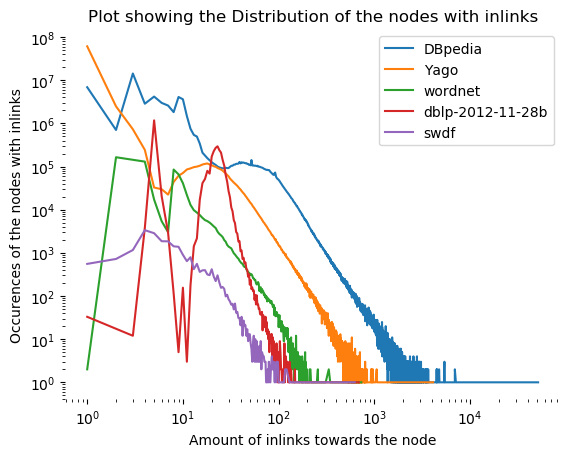
\includegraphics[width=0.33\textwidth]{images/figure4.png}
	}
	\subfloat[The distribution of outdegree over all nodes.\label{fig:outdegree}]{%
		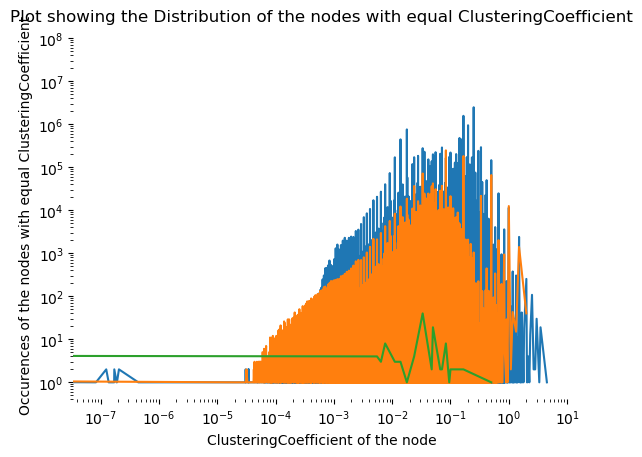
\includegraphics[width=0.33\textwidth]{images/figure5.png}
	}
	\subfloat[The distribution of the Clustering Coefficient over all nodes.\label{fig:Coeff}]{%
		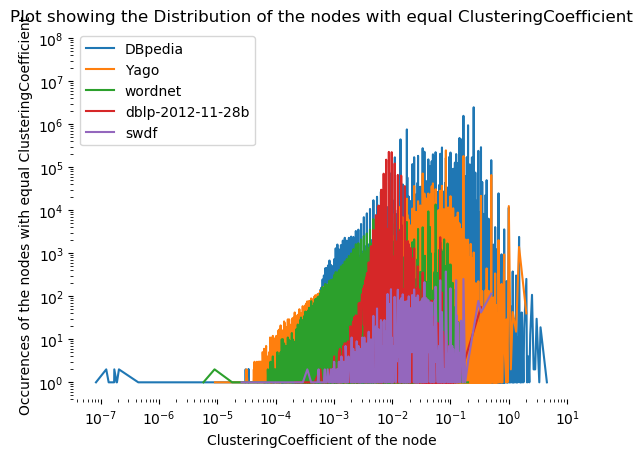
\includegraphics[width=0.33\textwidth]{images/figure6.png}
	}
	\vspace{\floatsep}
	\subfloat[The distribution of indegree over all nodes of the sample.\label{fig:indegreeSample}]{%
		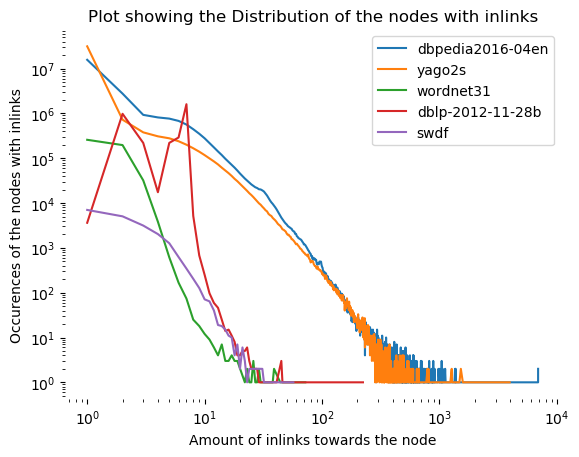
\includegraphics[width=0.33\textwidth]{images/Samplefigure4.png}
	}
	\subfloat[The distribution of outdegree over all nodes of the sample.\label{fig:outdegreeSample}]{%
		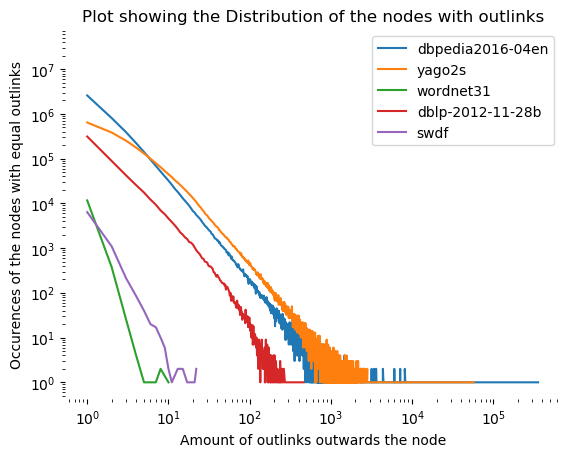
\includegraphics[width=0.33\textwidth]{images/Samplefigure5.png}
	}
	\subfloat[The distribution of the Clustering Coefficient over all nodes of the sample.\label{fig:CoeffSample}]{%
		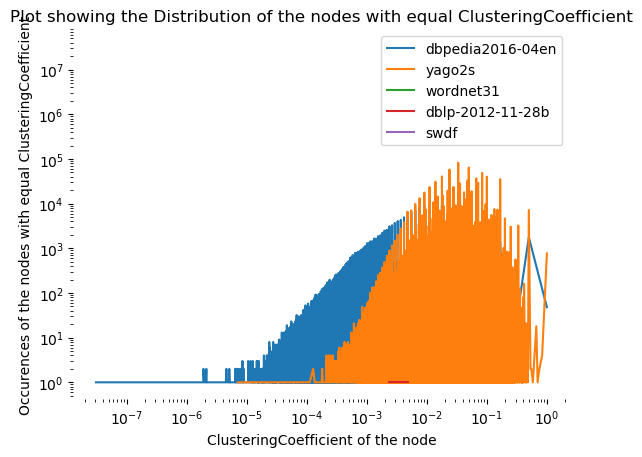
\includegraphics[width=0.33\textwidth]{images/Samplefigure6.png}
	}
	\caption{Figures showing several statistics about graphs.}
	\label{fig:GraphStats}
\end{figure}


\begin{figure}[ht]
	\centering
	\subfloat[Plot showing the Distribution of size.\label{fig:Size}]{%
		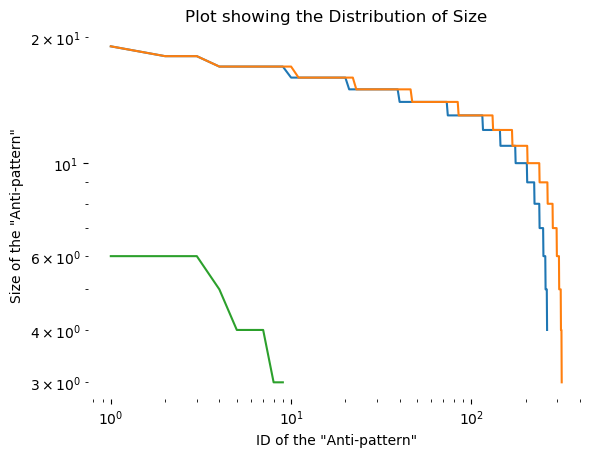
\includegraphics[width=0.33\textwidth]{images/figure1.png}
	}
	\subfloat[Plot showing the Distribution of occurrences.\label{fig:SizeSample}]{%
		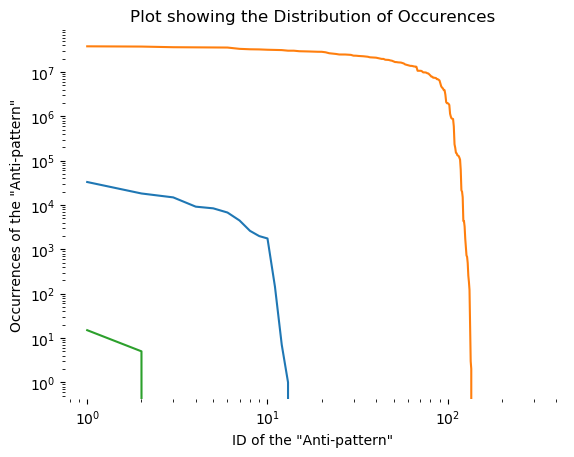
\includegraphics[width=0.33\textwidth]{images/figure2.png}
	}
	\subfloat[Plot showing the Distribution of occurrences.\label{fig:SizeSample2}]{%
		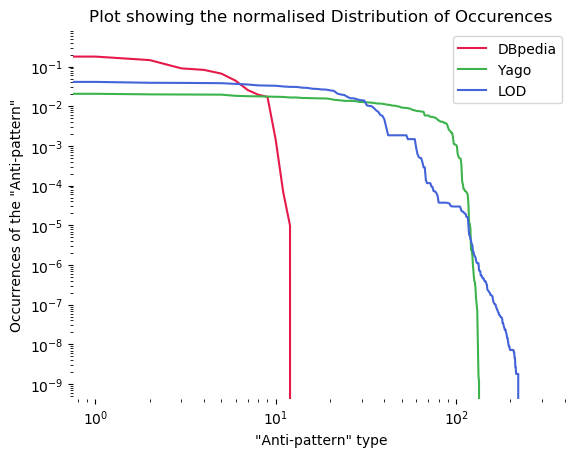
\includegraphics[width=0.33\textwidth]{images/figure3.png}
	}
	\caption{Figures showing several statistics about the Anti patterns.}
	\label{fig:AntipatternStats}
\end{figure}

\newpage


\chapter{Conclusion}\label{Conclusion}
This work we introduced three contributions to the field. 
The first contribution is the formal definition of an `anti-pattern'. In this work, we describe an anti-pattern as a minimal set of uninstantiated basic triple patterns that match an inconsistent subgraph in a knowledge graph. The advantage of converting justifications of contradictions in `anti-patterns' is that now we can use `anti-patterns' to locate contradictions in other knowledge graphs. Transferring knowledge about contradictions from one graph to the next was not easy with only justifications, but the `anti-patterns' solve this. 
Secondly, the generalisation saves the information space, as several justifications can be mapped onto a single `anti-pattern', and retrieving the justification from the knowledge graph can now be done using a simple query. Now using the `anti-patterns' finding how inconsistent a knowledge graph is can be asked by using SPARQL. Although we can not prove that being devoid of `anti-patterns' will mean that the knowledge graph is consistent. We can say for sure that if there is an `anti-pattern' match, the knowledge graph is inconsistent, and how.  \\

The second contribution we introduce in this work is the extraction pipeline. The pipeline has been designed to extract `anti-patterns' from any natural knowledge graph. In this work, we show that we can extract all `anti-patterns' from the knowledge graphs in our experiments. However, we can not prove that our implemented method will extract all `anti-patterns'.\\ 

The final contribution in this work are the two implementations, knowledge graph analysis and knowledge graph sampling with respect to `anti-patterns'. For knowledge graph analysis, we can now give qualitative and quantitative information about a knowledge graph concerning its inconsistency. In our experiments, we show relevant statistics that can be found using the `anti-patterns'. Using the analysis tool everybody can now check their knowledge graph for relevant statistics about their knowledge graph. \\

Finally for knowledge graph sampling, we showed that knowledge graph sampling with respect to `anti-pattern' is possible. We demonstrated this by sampling knowledge graphs by random deletion. We showed that sampled knowledge graphs still have the same characteristics with original knowledge graphs.\\

We made both the toolkit for sampling and analysis, as well as the extraction pipeline available on github. <INSERT LINK>. We also provide a range of `anti-patterns' with their equivalent SPARQL query on <INSERT LINK>.
\textit{Future Work}. We observed that `anti-patterns' follow the same distribution in each of the large knowledge graphs. the Analysis of the `anti-patterns' also showed that most `anti-patterns' consist out of `rdfs:subclassOf' and `owl:equivalentClass'. `rdfs:range' and `rdfs:domain' do not occur in the `anti-patterns'.
We want to evaluate why `rdfs:range' and `rdfs:domain' do not occur in the `anti-patterns' and we would improve the generalisation of `anti-patterns', by creating more general types for `anti-patterns'. At the moment, we have only looked at the most common knowledge graphs. We would also like to investigate the lesser-known knowledge graphs, such that we can expand our knowledge about the `anti-patterns' that occur in less known ontologies or graphs. Which can give us more insights into all types of ontologies.\\

Returning to Blaise Pascal, while we can not prove that our `anti-patterns' give the answers to consistent knowledge graphs, and the lack of `anti-patterns' will mean that a knowledge graph is devoid of mistakes. `Anti-patterns' will help us understand how contradictions in a knowledge graph come to be, and we use them to make the knowledge graphs cleaner.

\newpage
\bibliographystyle{plain}
\bibliography{ThesisBib}


\end{document}